\documentclass[a4paper]{article}
\usepackage{amsmath}
\usepackage{amsfonts}
\usepackage{amsthm}
\usepackage{amsfonts}
\usepackage{physics}
\usepackage{xparse}
\usepackage{graphicx}
\usepackage{siunitx}
\begin{document}
\section*{1}
\subsection*{(i)}
\[\begin{aligned}
    \text{LHS}&=\pqty{\vb u\vdot\vb v+\abs{\vb u\cross\vb v}}^2\\
    &=\pqty{\abs{\vb u}\abs{\vb v}\cos\theta+\abs{\abs{\vb u}\abs{\vb v}\sin\theta\vu n}}^2\\
    &=\pqty{\cos\theta+\sin\theta}^2\\
    &=\cos^2\theta+2\cos\theta\sin\theta+\sin^2\theta\\
    &=1+\sin2\theta\\
    &=\text{RHS}\qed
\end{aligned}\]
\subsection*{(ii)}
\[\begin{aligned}
    \pqty{\vb u+\vb w}\vdot\vb v&=\pqty{\vb u+\vb w}\vdot\vb v\\
    k\vb v\vdot\vb v&=\vb u\vdot\vb v+\vb w\vdot\vb v\\
    k\abs{\vb v}^2&=\abs{\vb u}\abs{\vb v}\cos\theta+\abs{\vb w}\abs{\vb v}\cos\theta\\
    k&=\boxed{2\cos\theta}
\end{aligned}\]
\subsection*{(iii)}
\[k\in\boxed{(0,2)}\]
\section*{2}
\subsection*{(i)}
Let \(z=x+iy\).
\[\begin{aligned}
    \sqrt3\abs{z-i}&=\sqrt2\abs{z-1-2i}\\
    \sqrt3\abs{x+iy-i}&=\sqrt2\abs{x+iy-1-2i}\\
    3\abs{x+i\pqty{y-1}}^2&=2\abs{x-1+i\pqty{y-2}}^2\\
    3\pqty{x^2+\pqty{y-1}^2}&=2\pqty{\pqty{x-1}^2+\pqty{y-2}^2}\\
    3\pqty{x^2+y^2-2y+1}&=2\pqty{x^2-2x+1+y^2-4y+4}\\
    3\pqty{x^2+y^2-2y+1}&=2\pqty{x^2+y^2-2x-4y+5}\\
    3x^2+3y^2-6y+3&=2x^2+2y^2-4x-8y+10\\
    x^2+y^2+4x+2y&=7\\
    x^2+4x+4+y^2+2y+1&=7+4+1\\
    \pqty{x+2}^2+\pqty{y+1}^2&=\sqrt{12}\\
    \pqty{x-\pqty{-2}}^2+\pqty{y-\pqty{-1}}^2&=\pqty{\sqrt{12}}^2\qed\\
\end{aligned}\]
\subsection*{(ii)}
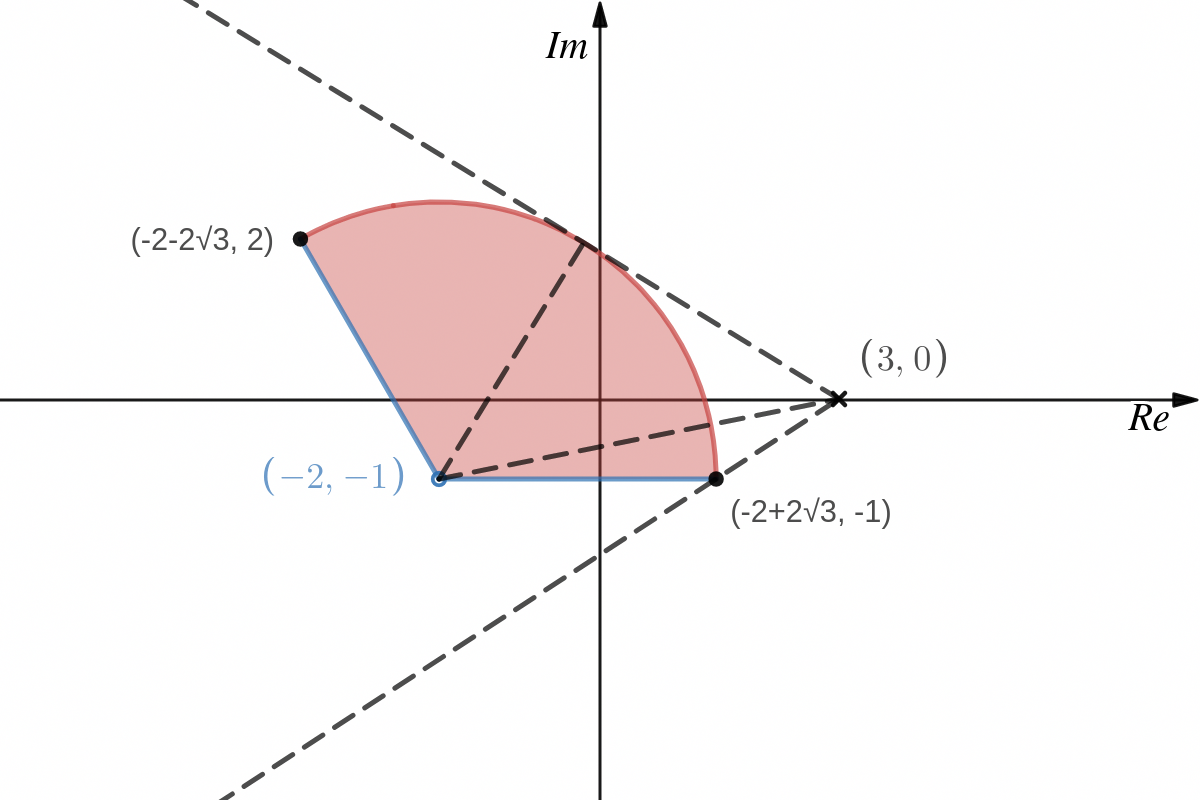
\includegraphics[width=\textwidth]{locus.png}
\[\arg\pqty{w-3}\in\boxed{\bqty{\cot[-1](5-\sqrt{12})-\pi,\cot^{-1}5-\csc^{-1}\frac{\sqrt{78}}6+\pi}}\]
\section*3
\subsection*{(i)}
\[\boxed{I\pqty{c,0}}\]
\subsection*{(ii)}
\[C_1:\boxed{x^2=4cy}\]
\subsection*{(iii)}
\[\begin{aligned}
    x^2&=4c\pqty{\frac c2}\\
    x^2&=2c^2\\
    x&=\pm c\sqrt2
\end{aligned}\]
\[\begin{aligned}
    AB&=40\\
    c\sqrt2-\pqty{-c\sqrt2}&=40\\
    2c\sqrt2&=40\\
    c&=\frac{20}{\sqrt2}\\
    c&=\boxed{10\sqrt2}
\end{aligned}\]
\[C_1:x^2=40\sqrt2y\]
\[\begin{aligned}
    C_2:x^2&=40\sqrt2\pqty{-\pqty{y-10\sqrt2}}\\
    &=40\sqrt2\pqty{10\sqrt2-y}\\
    &=800-40\sqrt2y\qed
\end{aligned}\]
\subsection*{(iv)}
\[\begin{aligned}
    x^2&=800-40\sqrt2y\\
    40\sqrt2y&=800-x^2\\
    y&=\frac{800-x^2}{40\sqrt2}\\
    \dv{y}{x}&=\frac{-2x}{40\sqrt2}\\
    \dv{y}{x}&=-\frac x{20\sqrt2}
\end{aligned}\]
\[\begin{aligned}
    A&=\int2\pi x\dd{s}\\
    &=2\pi\int_3^{20}x\sqrt{1+\pqty{\dv{y}{x}}^2}\dd{x}\\
    &=2\pi\int_3^{20}x\sqrt{1+\frac{x^2}{800}}\dd{x}\\
    &=800\pi\int_3^{20}\frac x{400}\sqrt{1+\frac{x^2}{800}}\dd{x}\\
    &=800\pi\eval{\frac23\pqty{1+\frac{x^2}{800}}^{\frac32}}_3^{20}\\
    &=\boxed{\SI{1374.25}{\centi\meter\squared}\,\text{{(2 dp)}}}
\end{aligned}\]
\subsection*{(v)}
\[\begin{aligned}
    V&=2\int_0^{20}2\pi x\pqty{y-5\sqrt2}\dd{x}-\int_0^32\pi x\pqty{10\sqrt2-y}\dd{x}\\
    &=4\pi\int_0^{20}x\pqty{\frac{800-x^2}{40\sqrt2}-5\sqrt2}\dd{x}-2\pi\int_0^3x\pqty{10\sqrt2-\frac{800-x^2}{40\sqrt2}}\dd{x}\\
    &=\boxed{\SI{8883.52}{\centi\meter\cubed}\,\text{{(2 dp)}}}
\end{aligned}\]
\section*4
\subsection*{(i)}
\[x_{t+1}=\frac{\Delta x}2+b=\frac{x_t-x_\text{intended}}2+b=\frac{x_t-0^\circ}2+b=\frac12x_t+b\qed\]
\subsection*{(ii)}
\[\begin{aligned}
    x_{t+1}+a&=B\pqty{x_t+a}\\
    x_{t+1}+a&=Bx_t+aB\\
    x_{t+1}&=Bx_t+aB-a\\
    x_{t+1}&=Bx_t+a(B-1)\\
\end{aligned}\]
\[\begin{cases}
    B=\frac12\\
    a(B-1)=b\implies a=-2b
\end{cases}\]
\[\begin{aligned}
    x_{t+1}&=\frac12x_t+b\\
    x_{t+1}-2b&=\frac12\pqty{x_t-2b}\\
    x_t-2b&=\pqty{\frac12}^t\pqty{x_0-2b}\\
    x_t&=\boxed{\frac{x_0-2b}{2^t}+2b}
\end{aligned}\]
\subsection*{(iii)}
\[\lim\limits_{t\to\infty}x_t=\lim\limits_{t\to\infty}\pqty{\frac{x_0-2b}{2^t}+2b}=2b\ne0^\circ\]
\subsection*{(iv)}
\[\begin{aligned}
    x_{t+1}&=2x_t+b\\
    x_{t+1}+b&=2\pqty{x_t+b}\\
    x_t+b&=2^t\pqty{x_0+b}\\
    x_t&=\boxed{2^t\pqty{x_0+b}-b}
\end{aligned}\]
\[\lim\limits_{t\to\infty}x_t=\lim\limits_{t\to\infty}\pqty{2^t\pqty{x_0+b}-b}=\infty\ne0^\circ\]
\subsection*{(iv)}
Peter's boat will spiral clockwise with an increasing rate.
\subsection*{(vi)}
First, Peter make sure that \(x_0=0^\circ\). Then, he can manually steer the boat such that it changes the direction of the boat by a constant \(b\) degrees towards the West.
\end{document}
